\section{Theory}

Light propagates through a medium at a lower velocity than in vaccum. This is described by the index of refraction of the medium

\begin{equation}
  \label{eq:refrInd}
  n = \frac{c_0}{v},
\end{equation}

where $c_0$ is the speed of light in vaccum and $v$ is the velocity in the medium\cite{phH}. By this, one can define the optical path length (OPL) as the length the light experiences. That is, if the light propagates through a medium of length $L$ and refractive index $n$, then the OPD will be

\begin{equation}
  \tn{OPD} = nL.
\end{equation}

The refractive index is thus a measure of how dense a material is and must therefore be proportional to the pressure. By increasing the pressure $P$ from vaccum, then

\begin{equation}
  \label{eq:refrVaccum}
  n-1 = \alpha \frac{\Delta P}{P_{atm}},
\end{equation}

where $P_{atm}$ is the atmospheric pressure and $\alpha$ is a proportionality constant\cite{nP}. Note that since $P$ is measured from vaccum then $\alpha=n-1$ at atmospheric pressure.

\subsection{The Michelson Interferometer}
A Michelson interferometer is built up by a laser beam being splitted into a reference leg $L_1$ and a signal leg $L_2$. The beams are then reflected back and reassembled at a sensor. A schematic sketch of this is found in Fig. \ref{fig:michelsonInterferometer}. If the beams are aligned correctly they will interfere with each ocher and constructive interference will occur if

\begin{equation}
\label{eq:interference}
  \tn{OPD} = N \lambda,
\end{equation}

where OPD is the optical path difference between the legs, $N$ is an integer and $\lambda$ is the wavelength of the laser beam.

\begin{figure}[H]
  \centering
  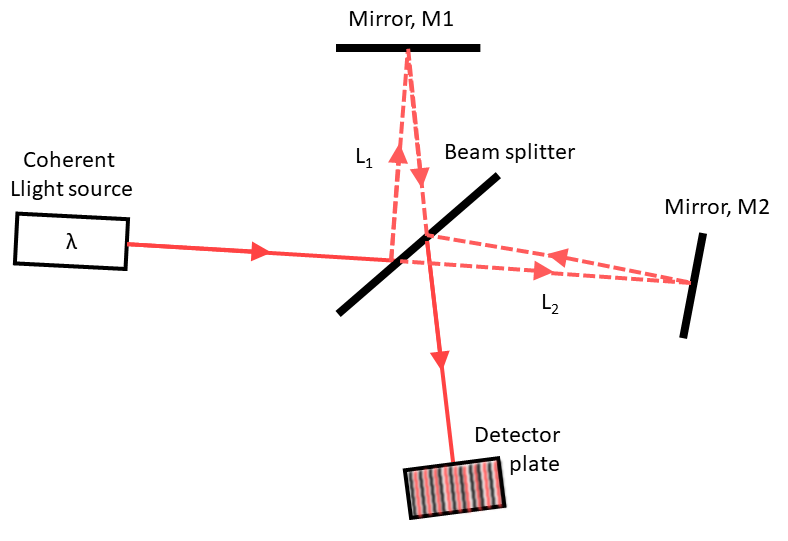
\includegraphics[width=0.8\textwidth]{Method.png}
  \caption{Principle of a Michelson interferometer. A coherent light source is split into two individual rays, these rays are reflected onto two mirrors and joined togheter again. When aligned properly an interference pattern can be observed at a detector plate.}
  \label{fig:michelsonInterferometer}
\end{figure}

\subsection{Method}

If a gas chamber of length $d$ is put on the sensor leg as shown in Fig. \ref{fig:experimentalSetup} the the OPD can be found as

\begin{equation}
  \label{eq:OPD}
  \tn{OPD} = 2\tn{OPL}_{L_2} - 2\tn{OPL}_{L_1} = 2nd + \tn{const.}
\end{equation}

Using the interference condition Eq. \eqref{eq:interference} this can be reduced to

\begin{equation}
\label{eq:fringes}
  N \lambda = 2nd + \tn{const.}
\end{equation}

Instead of counting the absolute number of interference maxima, called fringes, one can count the number of fringes that appear when changing the refractive index of the sample. Thus a change of $N$ corresponds to a change in $n$ and Eq. \ref{eq:fringes} yields

\begin{equation}
\label{eq:delta}
  \Delta N \lambda = 2d \Delta n.
\end{equation}

If one measures the number of fringes appearing when increasing the pressure of the gas from vaccum one can make use of Eq. \eqref{eq:refrVaccum} to reformulate Eq. \ref{eq:delta} and obtain

\begin{equation}
\label{eq:slope}
  \Delta N = \frac{2d\alpha}{\lambda P_{atm}} \Delta P.
\end{equation}

Thus, by continuously increasing the pressure of a gas from vaccum and counting how many fringes that has passed a sensor one can find the $\alpha$ from the slope of Eq. \eqref{eq:slope} and the refractive index from $n=\alpha+1$.
